\documentclass[14pt, letterpaper]{article}
\usepackage[utf8]{inputenc}
\usepackage{amsmath}
\usepackage{amssymb}
\usepackage{amsfonts}
\usepackage{listings}
\usepackage{xcolor}
\usepackage{dirtree}
\usepackage{caption}
\usepackage{hyperref}
\usepackage{setspace}
\usepackage{graphicx}
\usepackage[letterpaper, margin=1.5in, top=1.5in, bottom=1.5in]{geometry}
\graphicspath{{./images}}

\definecolor{gruv_red}{rgb}{0.8, 0.14118, 0.114}
\definecolor{gruv_blue}{rgb}{0.02745, 0.4, 0.4706}
\definecolor{gruv_yellow}{rgb}{0.84314, 0.6, 0.13}
\definecolor{gruv_orange}{rgb}{0.84, 0.3647, 0.055}
\definecolor{gruv_green}{rgb}{0.596, 0.59216, 0.102}
\definecolor{gruv_gray}{rgb}{0.5725, 0.5137, 0.4549}
\definecolor{gruv_aqua}{rgb}{0.4078, 0.6157, 0.4157}
\definecolor{gruv_purple}{rgb}{0.69412, 0.3843, 0.5255}

\hypersetup{
    colorlinks = true,
    citecolor=black,
    filecolor=black,
    linkcolor=black,
    urlcolor=gruv_aqua
}

\newcommand*{\QEDB}{\null\nobreak\hfill\ensuremath{\square}}%
\newcommand\tab[1][1cm]{\hspace*{#1}}
\newcommand\tabd[1][0.2cm]{\hspace*{#1}}

\lstset{
  language     = C++,
  frame        = tb,
  tabsize      = 4,
  basicstyle   = \footnotesize\ttfamily,
  keywordstyle = \color{gruv_blue}\textbf,
  commentstyle = \color{gruv_gray},
  stringstyle  = \color{gruv_green},
  other,
  columns      = fullflexible,
  numbers      = left,
  numberstyle  = \scriptsize\sffamily\color{gruv_gray},
  showstringspaces = false,
  float,
  %% new class
  classoffset   = 1, 
  otherkeywords = {>,<,.,::,(,),;,-,+,!,*,/,=,~},
  morekeywords  = {>,<,.,::,(,),;,-,+,!,*,/,=,~},
  keywordstyle  = \color{gruv_orange},
  classoffset   = 0,
}

\author{
        Joao Felipe Bianchi Curcio\\
        Jonas Edward Tashiro\\ 
        Luan Lopes Barbosa de Almeida\\ 
        Rafael Melloni Chacon Arnone\\ 
       }

\date{}
\title{
  \Huge{Mínimos Quadrados}\\[60.0mm]
}

\begin{document}

\maketitle
%\begin{center}
%\hypertarget{loretta}{}
%\end{center}
    
\newpage
\tableofcontents
\newpage

\section{Dependências}
\tab O programa foi escrito na linguagem C++ e faz utilização de API's e bibliotecas de  
Computação Gráfica para mostrar ao usuário, na forma de um plano cartesiano, a saída do 
problema dos Mínimos Quadrados, sendo que a biblioteca para "plotar" o gráfico foi a
biblioteca ImGui.\\[3.0mm] 
\tab A API utilizada para renderizar o plano cartesiano foi o Open-GL, pois é uma API 
multiplataforma, podendo ser executado em ambientes Linux e Windows. Além disto, 
algumas bibliotecas foram utilizadas para inicializar a API e facilitar a criação de 
janelas no Sistema Operacional, estas são, respectivamente, GLEW e GLFW.\\[3.0mm] 
\tab Abaixo fornecemos links de tutoriais para instalação das dependências.\\[3.0mm] 
\subsection{Windows:}
\tab Segue um vídeo demonstrando os passos necessários para instalação na plataforma.
\begin{center}
  \url{https://www.youtube.com/watch?v=OR4fNpBjmq8} 
\end{center}
\subsection{Linux(Distro-Ubuntu):}
\tab Primeiramente instale o ppa da biblioteca mesa para adquirir versões mais 
recentes da Biblioteca Mesa que possui o OpenGL.
\begin{center}
  \url{https://itsfoss.com/install-mesa-ubuntu/}
\end{center}
\tab E siga os passos a seguir para instalar GLEW e GLFW:
\begin{center}
  \url{https://medium.com/geekculture/a-beginners-guide-to-setup-opengl-in-linux-debian-2bfe02ccd1e}
\end{center}
\tab Após isto entre no terminal na pasta do projeto e escreva o comando make para compilar 
as bibliotecas e gerar o executável do programa. 
\subsection{Linux(Distro-Arch):}
\tab A instalação para distribuição Arch é elementar, basta fazer os seguintes comandos: 
\begin{center}
  \$ sudo pacman -Sy mesa \\
  \$ sudo pacman -Sy glfw \\
  \$ sudo pacman -Sy make 
\end{center}
\tab Após isto entre no terminal na pasta do projeto e escreva o comando make para compilar 
as bibliotecas e gerar o executável do programa. 

\section{Organização de Pastas}
\dirtree{%
  .1 /src/.
  .2 /imgui/.
  .2 {App.cpp}.
  .2 {lsq.h}.
  .2 {lsq.cpp}.
}

\section{Conteúdo dos Arquivos}

\begin{spacing}{2.5}
\end{spacing}

\begin{lstlisting}[caption=Makefile]
EXE = App
IMGUI_DIR = ./imgui
SOURCES = App.cpp lsq.cpp
SOURCES += $(IMGUI_DIR)/imgui.cpp $(IMGUI_DIR)/imgui_demo.cpp
SOURCES += $(IMGUI_DIR)/imgui_draw.cpp $(IMGUI_DIR)/imgui_tables.cpp $(IMGUI_DIR)/imgui_widgets.cpp
SOURCES += $(IMGUI_DIR)/implot_items.cpp $(IMGUI_DIR)/implot.cpp
SOURCES += $(IMGUI_DIR)/imgui_impl_glfw.cpp $(IMGUI_DIR)/imgui_impl_opengl3.cpp
SOURCES += $(IMGUI_DIR)/imgui_stdlib.cpp
OBJS = $(addsuffix .o, $(basename $(notdir $(SOURCES))))
UNAME_S := $(shell uname -s)
LINUX_GL_LIBS = -lGL -lGLEW

CXXFLAGS = -std=c++11 -I$(IMGUI_DIR)
CXXFLAGS += -g -Wall -Wformat -pthread
LIBS =

##---------------------------------------------------------------------
## BUILD FLAGS PER PLATFORM
##---------------------------------------------------------------------

ifeq ($(UNAME_S), Linux) #LINUX
	ECHO_MESSAGE = "Linux"
		LIBS += $(LINUX_GL_LIBS) `pkg-config --static --libs glfw3`

	CXXFLAGS += `pkg-config --cflags glfw3`
		CFLAGS = $(CXXFLAGS)
endif

ifeq ($(OS), Windows_NT)
	ECHO_MESSAGE = "MinGW"
		LIBS += -lglfw3 -lgdi32 -lopengl32 -limm32

	CXXFLAGS += -L$(shell pwd)
	CXXFLAGS += `pkg-config --cflags glfw3`
		CFLAGS = $(CXXFLAGS)
endif

##---------------------------------------------------------------------
## BUILD RULES
##---------------------------------------------------------------------

%.o:%.cpp
		$(CXX) $(CXXFLAGS) -c -o $@ $<

%.o:$(RENDER)/%.cpp
		$(CXX) $(CXXFLAGS) -c -o $@ $<
	
%.o:$(IMGUI_DIR)/%.cpp
		$(CXX) $(CXXFLAGS) -c -o $@ $<

%.o:$(STBI)/%.cpp
		$(CXX) $(CXXFLAGS) -c -o $@ $<

all: $(EXE)
		@echo Build complete for $(ECHO_MESSAGE)

$(EXE): $(OBJS)
		$(CXX) -o $@ $^ $(CXXFLAGS) $(LIBS)

clean:
		rm -f $(EXE) $(OBJS)
\end{lstlisting}

\begin{spacing}{2.5}
\end{spacing}

\begin{lstlisting}[caption=App.cpp]
#include <GL/glew.h>
#include <GLFW/glfw3.h>
#include "imgui/imgui.h"
#include "imgui/imgui_stdlib.h"
#include "imgui/imgui_impl_glfw.h"
#include "imgui/imgui_impl_opengl3.h"
#include "imgui/implot.h"
#include "imgui/implot_internal.h"
#include <array>
#include <cstddef>
#include <string>
#include <utility>
#include <vector>
#include <iostream>
#include <algorithm>
#include "lsq.h"
#define glsl_version "#version 420"

void Initialize_GLFW();
void Initialize_GLEW();
void Initialize_ImGui();
void Cleanup_OpenGL();
void Cleanup_ImGui();
void display();

int main()
{
    Initialize_GLFW();
    Initialize_ImGui();

    GLFWwindow* window = glfwCreateWindow(1920, 1080, "Least Squares Method", NULL, NULL);
    if(window == NULL)
    {
        std::cout<<"Failed to Initialize Window\n";
        glfwTerminate();
    }

    glfwMakeContextCurrent(window);
    glfwSwapInterval(1);
    ImGui_ImplGlfw_InitForOpenGL(window, true);
    ImGui_ImplOpenGL3_Init(glsl_version);
    Initialize_GLEW();

    glClearColor(0.07f, 0.13f, 0.17f, 1.0f);

    while (!glfwWindowShouldClose(window))
    {
        glClear(GL_COLOR_BUFFER_BIT);
        ImGui_ImplOpenGL3_NewFrame();
        ImGui_ImplGlfw_NewFrame();
        ImGui::NewFrame(); 
        display();
        ImGui::Render();
        ImGui_ImplOpenGL3_RenderDrawData(ImGui::GetDrawData());
        glfwPollEvents();                     
        glfwSwapBuffers(window); 
    }

    Cleanup_ImGui();
    Cleanup_OpenGL();

    return 0;
}

void Initialize_GLFW()
{
    if (!glfwInit())
    {
        std::cout << "Failed to Initialize GLFW\n";
        exit(EXIT_FAILURE);
    }

    glfwWindowHint(GLFW_CONTEXT_VERSION_MAJOR, 4);
    glfwWindowHint(GLFW_CONTEXT_VERSION_MINOR, 2);
    glfwWindowHint(GLFW_OPENGL_PROFILE, GLFW_OPENGL_CORE_PROFILE); // 3.2+ only
}

void Initialize_GLEW()
{
    /*Initialize GLEW Library*/
    if (glewInit() != GLEW_OK)
    {
        glfwTerminate();
        exit(EXIT_FAILURE);
    }
}

void Initialize_ImGui()
{
    /*ImGUI Initialization*/
    IMGUI_CHECKVERSION();
    ImGui::CreateContext();
    ImPlot::CreateContext();
    ImGuiIO &io = ImGui::GetIO();
    (void)io;
    ImGui::StyleColorsDark();
}

void Cleanup_OpenGL()
{
    glfwTerminate();
}

void Cleanup_ImGui()
{
    // Cleanup
    ImGui_ImplOpenGL3_Shutdown();
    ImGui_ImplGlfw_Shutdown();
    ImPlot::DestroyContext();
    ImGui::DestroyContext();
}

void display()
{
    static int precision = 3;
    static int number = 5;
    static std::string ids[20];
    static std::string expression;
    static std::string info;
    static std::array<float, 2> x_axis;
    static std::array<float, 2> y_axis;
    static std::vector<float> points_x_axis;
    static std::vector<float> points_y_axis;
    static std::vector<std::pair<float, float>> coord_pairs = 
        {{2.0f,5.0f},{4.0f,4.0f},{6.0f,8.0f},{8.0f,6.0f},{10.0f,12.0f}};
    static lsq solver(coord_pairs);
    static bool setup = true;   // used only once

    if(setup)
    {
        for (int i = 0; i < 20; i++)
        {
            ids[i] = 'P';
            ids[i] += std::to_string(i + 1);
            ids[i] += "(x,y)";
        }
        solver.get_fuction_expr(expression, precision);
        solver.generate_graph(x_axis, y_axis, points_x_axis, points_y_axis, coord_pairs);
        solver.get_info(info, precision);
        setup = false;
    }

    ImGui::Begin("Opcoes", NULL, ImGuiWindowFlags_NoCollapse);
    ImGui::SliderInt("Precisao", &precision, 2, 10);
    ImGui::SliderInt("Numero de Pares", &number, 3, 20);

    while (coord_pairs.size() <  (std::size_t) number)
        coord_pairs.push_back(std::make_pair(1.0f, 1.0f));
    if ((std::size_t) number < coord_pairs.size())
        coord_pairs.resize(number);

    ImGui::Spacing();
    if(ImGui::TreeNode("Coordenadas"))
    {
        for (int i = 0; i < number; i++)
            ImGui::InputFloat2(ids[i].data(), (float*) &coord_pairs[i]); 
        ImGui::TreePop();
    }

    if(ImGui::Button("Atualizar Dados"))
    {
        solver.associate_data(coord_pairs);
        solver.generate_graph(x_axis, y_axis, points_x_axis, points_y_axis, coord_pairs);
        solver.get_fuction_expr(expression, precision);
        solver.get_info(info, precision);
    }

    if(ImPlot::BeginPlot("Grafico"))
    {
        ImPlot::PlotLine(expression.data(), x_axis.data(), y_axis.data(),x_axis.size());
        ImPlot::PlotScatter("Pares de Pontos", points_x_axis.data(),points_y_axis.data(),
                            points_x_axis.size());
        ImPlot::EndPlot();
    }

    ImGui::InputTextMultiline("Info", &info, ImVec2(0,0), ImGuiInputTextFlags_ReadOnly);

    ImGui::End();
}
\end{lstlisting}

\begin{spacing}{2.5}
\end{spacing}

\begin{lstlisting}[caption=lsq.h]
#include <array>
#include <cstddef>
#include <string>
#include <utility>
#include <vector>

using pair_iter = std::vector<std::pair<float, float>>::iterator;

struct lsq
{
    /* data */
        std::array<float, 2> line;
        float pearson;
        float pearson_sqr;
        float sum_x;
        float sum_y;
        float sum_xx;
        float sum_xy;
        std::size_t n_pairs;
    /* methods */
        lsq();
        lsq(std::vector<std::pair<float, float>> &point_data);
        void generate_graph(std::array<float,2> &x_axis, std::array<float,2> &y_axis,
                        std::vector<float> &x_axis_points, std::vector<float> &y_axis_points,
                        std::vector<std::pair<float, float>> &point_data);
        void associate_data(std::vector<std::pair<float, float>> &point_data);
        void get_fuction_expr(std::string& expression, int precision);
        void get_info(std::string& lsq_info, int precision);

        private:
        pair_iter find_max_x(const pair_iter& begin, const pair_iter&end);
        pair_iter find_min_x(const pair_iter& begin, const pair_iter&end);
        pair_iter find_max_y(const pair_iter& begin, const pair_iter&end);
        pair_iter find_min_y(const pair_iter& begin, const pair_iter&end);
};
\end{lstlisting}

\begin{spacing}{2.5}
\end{spacing}

\begin{lstlisting}[caption=lsq.cpp]
#include "lsq.h"
#include <ios>
#include <sstream>
#include <string>
#include <type_traits>
#include <utility>
#include <cmath>
#include <iomanip>


lsq::lsq()
{
    /* f(x) = ax + b, na qual a: line[1] e b: line[0]*/
    line[0] = 1.0f;
    line[1] = 0.0f;
    pearson = pearson_sqr =  sum_x = sum_y
    = sum_xx =  sum_xy = n_pairs = 0.0f;
}

lsq::lsq(std::vector<std::pair<float, float>> &point_data)
{
    associate_data(point_data);
}

void lsq::associate_data(std::vector<std::pair<float, float>> &point_data)
{
    #define x first
    #define y second 

    float mean_x{}, mean_y{}, desv_x, desv_y, sum_yy{};
    sum_x = sum_y = sum_xx = sum_xy = 0.0f;

    for (auto elem : point_data)
    {
        sum_x += elem.x;
        sum_y += elem.y;
        sum_xy += elem.x * elem.y;
        sum_xx += elem.x * elem.x;
        sum_yy += elem.y * elem.y;
    }

    n_pairs = point_data.size();
    mean_x = sum_x / static_cast<float>(n_pairs);
    mean_y = sum_y / static_cast<float>(n_pairs);
    pearson = sum_xy / static_cast<float>(n_pairs);
    pearson = pearson - mean_x * mean_y; // Cov(mean_x, mean_y)
    desv_x = sum_xx / static_cast<float>(n_pairs) - mean_x * mean_x;
    desv_y = sum_yy / static_cast<float>(n_pairs) - mean_y * mean_y;
    pearson /= std::sqrt(desv_x * desv_y);
    pearson_sqr = pearson * pearson;
    float denum = static_cast<float>(n_pairs) * sum_xx - sum_x * sum_x;
    
    line[0] = (static_cast<float>(n_pairs) * sum_xy - sum_x * sum_y) / denum;
    line[1] = (sum_y * sum_xx - sum_x * sum_xy) / denum; 
}

void lsq::get_fuction_expr(std::string& expression, int precision)
{
    std::stringstream stream;
    stream << std::fixed << std::setprecision(precision) << line[0];
    expression.clear();
    expression = stream.str();
    expression += " * x + ";
    stream.str("");
    stream << line[1];
    expression += stream.str();
}

void lsq::get_info(std::string &lsq_info, int precision)
{
    std::stringstream stream;
    lsq_info.clear();
    stream << std::fixed << std::setprecision(precision) << pearson;
    lsq_info = "Coeficiente de correlacao de Pearson = ";
    lsq_info += stream.str();
    stream.str("");
    stream << pearson_sqr;
    lsq_info += "\nCoeficiente de determinacao de Pearson = ";
    lsq_info += stream.str();
    stream.str("");
    stream << sum_x;
    lsq_info += "\nsum_x = ";
    lsq_info += stream.str();
    stream.str("");
    stream << sum_y;
    lsq_info += "\nsum_y = ";
    lsq_info += stream.str();
    stream.str("");
    stream << sum_xy;
    lsq_info += "\nsum_xy = ";
    lsq_info += stream.str();
    stream.str("");
    stream << sum_xx;
    lsq_info += "\nsum_xx = ";
    lsq_info += stream.str();
    lsq_info += "\nNumero de Pares = ";
    lsq_info += std::to_string(n_pairs);
}

void lsq::generate_graph(std::array<float,2> &x_axis, std::array<float,2> &y_axis,
                        std::vector<float> &x_axis_points, std::vector<float> &y_axis_points,
                        std::vector<std::pair<float, float>> &point_data)
{
    float max_x = (*find_max_x(point_data.begin(), point_data.end())).first;
    float min_x = (*find_min_x(point_data.begin(), point_data.end())).first;

    x_axis[0] = min_x - 10.0f;
    y_axis[0] = line[0] * x_axis[0] + line[1];
    x_axis[1] = max_x + 10.0f;
    y_axis[1] = line[0] * x_axis[1] + line[1];

    x_axis_points.clear();
    y_axis_points.clear();
    for (auto elem : point_data)
    {
        x_axis_points.push_back(elem.first);
        y_axis_points.push_back(elem.second);
    }
}

pair_iter lsq::find_max_x(const pair_iter& begin, const pair_iter&end)
{
    pair_iter found = begin;
    pair_iter b_iter = begin;
    pair_iter e_iter = end;
    while (b_iter != e_iter)
    {
        if((*found).first < (*b_iter).first)
            found = b_iter;
        b_iter++;    
    }
    return found;
}

pair_iter lsq::find_min_x(const pair_iter& begin, const pair_iter&end)
{
    pair_iter found = begin;
    pair_iter b_iter = begin;
    pair_iter e_iter = end;
    while (b_iter != e_iter)
    {
        if((*found).first > (*b_iter).first)
            found = b_iter;
        b_iter++;    
    }
    return found;
}

pair_iter lsq::find_max_y(const pair_iter& begin, const pair_iter&end)
{
    pair_iter found = begin;
    pair_iter b_iter = begin;
    pair_iter e_iter = end;
    while (b_iter != e_iter)
    {
        if((*found).second < (*b_iter).second)
            found = b_iter;
        b_iter++;    
    }
    return found;
}

pair_iter lsq::find_min_y(const pair_iter& begin, const pair_iter&end)
{
    pair_iter found = begin;
    pair_iter b_iter = begin;
    pair_iter e_iter = end;
    while (b_iter != e_iter)
    {
        if((*found).second > (*b_iter).second)
            found = b_iter;
        b_iter++;    
    }
    return found;
}   
\end{lstlisting}
\section{Exemplo}
\tab A seguir demonstramos um exemplo extraído do 2 Volume do livro do Um Curso de Cálculo, 
capítulo 17 página 373, do autor Guidorizzi.

\begin{center}
  \captionof{table}{Entrada}
  \begin{tabular}{|c | c | c | c | c | c|}
    \hline
    x & 2.0 & 4.0 & 6.0 & 8.0 & 10.0\\ 
    \hline
    y & 5.0 & 4.0 & 8.0 & 6.0 & 12.0\\ 
    \hline
  \end{tabular}
\end{center}

\begin{spacing}{2.5}
\end{spacing}

\begin{center}
  \textbf{Exemplo de execução do programa\\[5.0mm]}
  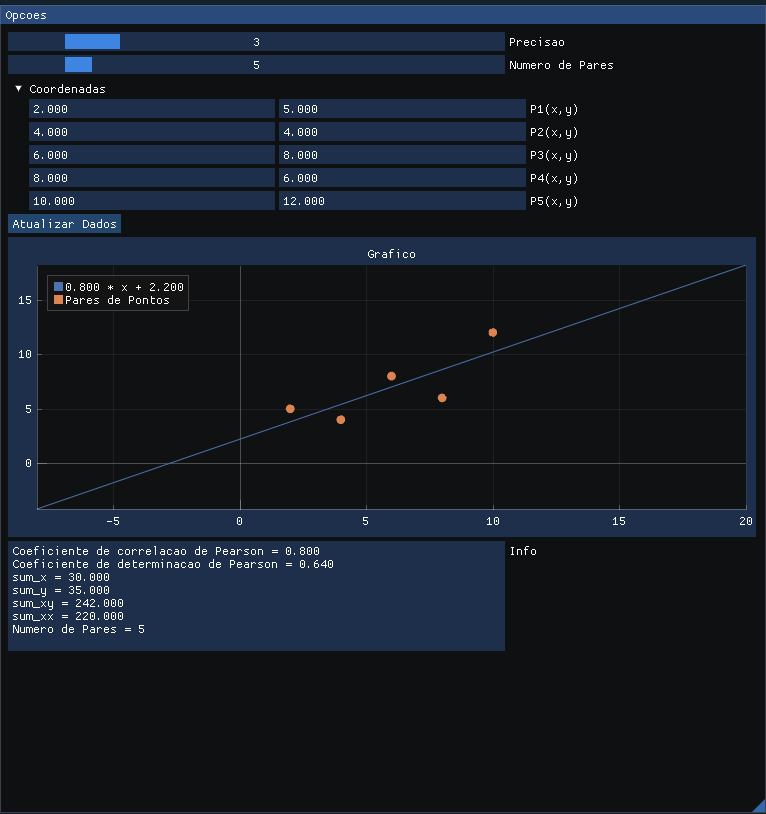
\includegraphics[scale=0.4]{exemplo}
\end{center}
\end{document}
